

%%%%%%%%%%%%%%%%%%%%%%%%%%%%%%%%%%%%%%%%%%%%%%%%%%%%%%%%%%%%%%%%%%%%%
%% This is a (brief) model paper using the achemso class
%% The document class accepts keyval options, which should include
%% the target journal and optionally the manuscript type.
%%%%%%%%%%%%%%%%%%%%%%%%%%%%%%%%%%%%%%%%%%%%%%%%%%%%%%%%%%%%%%%%%%%%%
\documentclass[journal=jacsat,manuscript=article]{achemso}
\usepackage{amssymb}
\usepackage{amsmath}
\usepackage{comment}
%%%%%%%%%%%%%%%%%%%%%%%%%%%%%%%%%%%%%%%%%%%%%%%%%%%%%%%%%%%%%%%%%%%%%
%% Place any additional packages needed here.  Only include packages
%% which are essential, to avoid problems later.
%%%%%%%%%%%%%%%%%%%%%%%%%%%%%%%%%%%%%%%%%%%%%%%%%%%%%%%%%%%%%%%%%%%%%
\usepackage{multirow}
\usepackage{chemformula} % Formula subscripts using \ch{}
\usepackage[T1]{fontenc} % Use modern font encodings
%%%%%%%%%%%%%%%%%%%%%%%%%%%%%%%%%%%%%%%%%%%%%%%%%%%%%%%%%%%%%%%%%%%%%
%% If issues arise when submitting your manuscript, you may want to
%% un-comment the next line.  This provides information on the
%% version of every file you have used.
%%%%%%%%%%%%%%%%%%%%%%%%%%%%%%%%%%%%%%%%%%%%%%%%%%%%%%%%%%%%%%%%%%%%%
%%\listfiles

%%%%%%%%%%%%%%%%%%%%%%%%%%%%%%%%%%%%%%%%%%%%%%%%%%%%%%%%%%%%%%%%%%%%%
%% Place any additional macros here.  Please use \newcommand* where
%% possible, and avoid layout-changing macros (which are not used
%% when typesetting).
%%%%%%%%%%%%%%%%%%%%%%%%%%%%%%%%%%%%%%%%%%%%%%%%%%%%%%%%%%%%%%%%%%%%%
\newcommand*\mycommand[1]{\texttt{\emph{#1}}}

\setkeys{acs}{maxauthors=10}
\setkeys{acs}{etalmode=truncate}

\usepackage{float} 
\usepackage{tikz}
\usepackage{multirow}
\usepackage{longtable}
%%\usepackage{bm}
\usepackage{caption}
\usepackage{arydshln}
\usepackage{xr} % for cross reference


%%%%%%%%%%%%%%%%%%%%%%%%%%%% Barnabas' Added packages %%%%%%%%%%%%%
\usepackage{verbatim} %for easy writing of multi-line comments
\usepackage{csvsimple}
\usepackage{bm}
\usepackage{epstopdf}
\usepackage{url}
\usepackage{hyperref}
\usepackage{array}

\graphicspath{ {./images/} }
%%%\usepackage{array}
%%%%%%%%%%%%%%%%%%%%%%%%%%%%


%%%%%%%%%%%%%%%%%%%%%%%%%%% KJ commands
\usepackage{xcolor}
\newcommand{\kjnote}[1]{{\color{blue} (#1)}}
\newcommand{\mcnote}[1]{{\color{purple} (#1)}}
\newcommand{\kjtodo}[1]{{\color{red} (#1)}}
\newcommand{\alltodo}[1]{{\color{cyan} (#1)}}
\newcommand{\reals}{\ensuremath{\mathbb{R}}}
\newcommand{\xvec}{\ensuremath{\mathbf{x}}}
\newcommand{\MW}{\ensuremath{\text{M.W}}}
\newcommand{\Ygc}[1][]{\ensuremath{y_{\text{GC}_{#1}}}}
\newcommand{\Ygcvec}[1][]{\ensuremath{\mathbf{y}_{\text{GC}_{#1}}}}
\newcommand{\yexpvec}[1][]{\ensuremath{\mathbf{y}_{\text{exp}_{#1}}}}
\newcommand{\yexp}[1][]{\ensuremath{y_{\text{exp}_{#1}}}}
\usepackage{setspace}
\doublespacing % needed for proper spacing of piecewise functions

% this is for cross reference 
\makeatletter
\newcommand*{\addFileDependency}[1]{% argument=file name and extension
  \typeout{(#1)}
  \@addtofilelist{#1}
  \IfFileExists{#1}{}{\typeout{No file #1.}}
}
\makeatother

\newcommand*{\myexternaldocument}[1]{%
    \externaldocument{#1}%
    \addFileDependency{#1.tex}%
    \addFileDependency{#1.aux}%
}
\myexternaldocument{SI}

%%%%%%%%%%%%%%%%%%%%%%%%%%%%%%%%%%%%%%%%%%%%%%%%%%%%%%%%%%%%%%%%%%%%%
%% Meta-data block
%% ---------------
%% Each author should be given as a separate \author command.
%%
%% Corresponding authors should have an e-mail given after the author
%% name as an \email command. Phone and fax numbers can be given
%% using \phone and \fax, respectively; this information is optional.
%%
%% The affiliation of authors is given after the authors; each
%% \affiliation command applies to all preceding authors not already
%% assigned an affiliation.
%%
%% The affiliation takes an option argument for the short name.  This
%% will typically be something like "University of Somewhere".
%%
%% The \altaffiliation macro should be used for new address, etc.
%% On the other hand, \alsoaffiliation is used on a per author basis
%% when authors are associated with multiple institutions.
%%%%%%%%%%%%%%%%%%%%%%%%%%%%%%%%%%%%%%%%%%%%%%%%%%%%%%%%%%%%%%%%%%%%%
\usepackage[symbol]{footmisc}
\author{Barnabas P. Agbodekhe}
\author{Dinis O. Abranches}
\author{Montana N. Carlozo}
\author{Kyla D. Jones}
\author{Alexander W.~Dowling}
\author{Edward J. Maginn}
\email{ed@nd.edu}
%\phone{+123 (0)123 4445556}
%\fax{+123 (0)123 4445557}
\affiliation[University of Notre Dame]
{Department of Chemical and Biomolecular Engineering, University of Notre Dame, Notre Dame, IN 46556, USA}
%\alsoaffiliation[Second University]{Department of Chemistry, Second University, Nearby Town}

%%%%%%%%%%%%%%%%%%%%%%%%%%%%%%%%%%%%%%%%%%%%%%%%%%%%%%%%%%%%%%%%%%%%%
%% The document title should be given as usual. Some journals require
%% a running title from the author: this should be supplied as an
%% optional argument to \title.
%%%%%%%%%%%%%%%%%%%%%%%%%%%%%%%%%%%%%%%%%%%%%%%%%%%%%%%%%%%%%%%%%%%%%
\title[An \textsf{achemso}]
  {Synergy Between Group Contribution and Gaussian Process Regression Models for Simple, Generalizable, and Accurate Thermophysical Property Prediction}

%%%%%%%%%%%%%%%%%%%%%%%%%%%%%%%%%%%%%%%%%%%%%%%%%%%%%%%%%%%%%%%%%%%%%
%% Some journals require a list of abbreviations or keywords to be
%% supplied. These should be set up here, and will be printed after
%% the title and author information, if needed.
%%%%%%%%%%%%%%%%%%%%%%%%%%%%%%%%%%%%%%%%%%%%%%%%%%%%%%%%%%%%%%%%%%%%%
\abbreviations{GC}
\keywords{Group Contribution, thermophysical properties}

%%%%%%%%%%%%%%%%%%%%%%%%%%%%%%%%%%%%%%%%%%%%%%%%%%%%%%%%%%%%%%%%%%%%%
%% The manuscript does not need to include \maketitle, which is
%% executed automatically.
%%%%%%%%%%%%%%%%%%%%%%%%%%%%%%%%%%%%%%%%%%%%%%%%%%%%%%%%%%%%%%%%%%%%%
\begin{document}

\sloppy  % stops long words from running over the margin
%%%%%%%%%%%%%%%%%%%%%%%%%%%%%%%%%%%%%%%%%%%%%%%%%%%%%%%%%%%%%%%%%%%%%
%% The "tocentry" environment can be used to create an entry for the
%% graphical table of contents. It is given here as some journals
%% require that it is printed as part of the abstract page. It will
%% be automatically moved as appropriate.
%%%%%%%%%%%%%%%%%%%%%%%%%%%%%%%%%%%%%%%%%%%%%%%%%%%%%%%%%%%%%%%%%%%%%

%%%%%%%%%%%%%%%%%% TO BE EDITED %%%%%%%%%%%%%%%%%%%%

%\begin{tocentry}
%\begin{figure}[H]
%    \centering
%    \includegraphics[width=8cm,scale=0.5]{TOC_graphic_abstract_0526_1344.eps}
%    %\caption{}
%    \label{fig:toc}
%\end{figure}
% Assessment of predictive performance and ranking of FFs using properties not used in FF tuning. 
%\end{tocentry}
%%%%%%%%%%%%%%%%%%%%%%%%%%%%%%%%%%%%%%%%%%%%%%%%%%%%%%%%%%%%%%%%%%%%%
%% The abstract environment will automatically gobble the contents
%% if an abstract is not used by the target journal.
%%%%%%%%%%%%%%%%%%%%%%%%%%%%%%%%%%%%%%%%%%%%%%%%%%%%%%%%%%%%%%%%%%%%%
\begin{abstract}
Abstract
\end{abstract}


%%%%%%%%%%%%%%%%%%%%%%%%%%%%%%%%%%%%%%%%%%%%%%%%%%%%%%%%%%%%%%%%%%%%%
%% Start the main part of the manuscript here.
%%%%%%%%%%%%%%%%%%%%%%%%%%%%%%%%%%%%%%%%%%%%%%%%%%%%%%%%%%%%%%%%%%%%%

\section{Introduction}


-Thermophysical property prediction is key to all material, and process development tasks with applications in many fields

-GC models

-The Joback and Reid GC model

-Limitations of GC models

- GP models

-Use of GP models as 'corrector' models

-The central idea: use GC predictions in GP models for improved property prediction

-How the rest of the paper is organized


\section{Methods}
\alltodo{standard in math is to remove equation numbers from all equations not referenced somewhere else in the text. Primary authors please either delete this comment if not standard for target journal or remind everyone to remove numbers from equations not referenced in the text at the end}
\subsection{Data Collection and Preparation}
\subsection{Joback and Reid GC Method}
\subsection{Data Pre-processing} \label{sec:preprocess}
%Analysis of feature vs label data and standardization (Montana and Kyla)
We begin the modeling creation process by thoroughly analyzing the trends in the data. Figures \ref{fig:Data_Vis_Disc} and \ref{fig:Data_Vis_Prop} demonstrate that the GC predictions and molecular weight are correlated with the experimental data for all properties of interest. Figure \ref{fig:Data_Vis_Disc} shows that the discrepancy between GC predictions and experimental data are zero and thus, linearly correlated for $H_{vap}$, $P_c$, $V_c$. This is desirable behavior as we would ideally like our GC model to be relatively unbiased. The GC models for $T_m$, $T_b$ and $T_c$ are much worse predictors of the experimental data and thus we observe a nonlinear trend indicated by nonzero trends in the discrepancy. Figure \ref{fig:Data_Vis_Prop} demonstrates correlation between molecular weight and the experimental data and GC predictions for $V_c$, $T_b$, and $T_m$. However the two-tail trend that we observe for the molecular weight correlations suggests that another descriptor should be added to fully explain the data. We observe that $H_{vap}$ does not have a strong correlation with molecular weight, and that $P_c$ exhibits a strong nonlinear trend suggesting that molecular weight is an excellent molecular descriptor for $P_c$ and subpar for $H_{vap}$. However, we note that multiple studies list a relationship between $H_{vap}$ and molecular weight and therefore conclude that molecular weight is an adequate molecular descriptor for all properties of interest. (todo: Barnabas add the studies you mentioned which support this)

\begin{figure}[H]
    \centering
    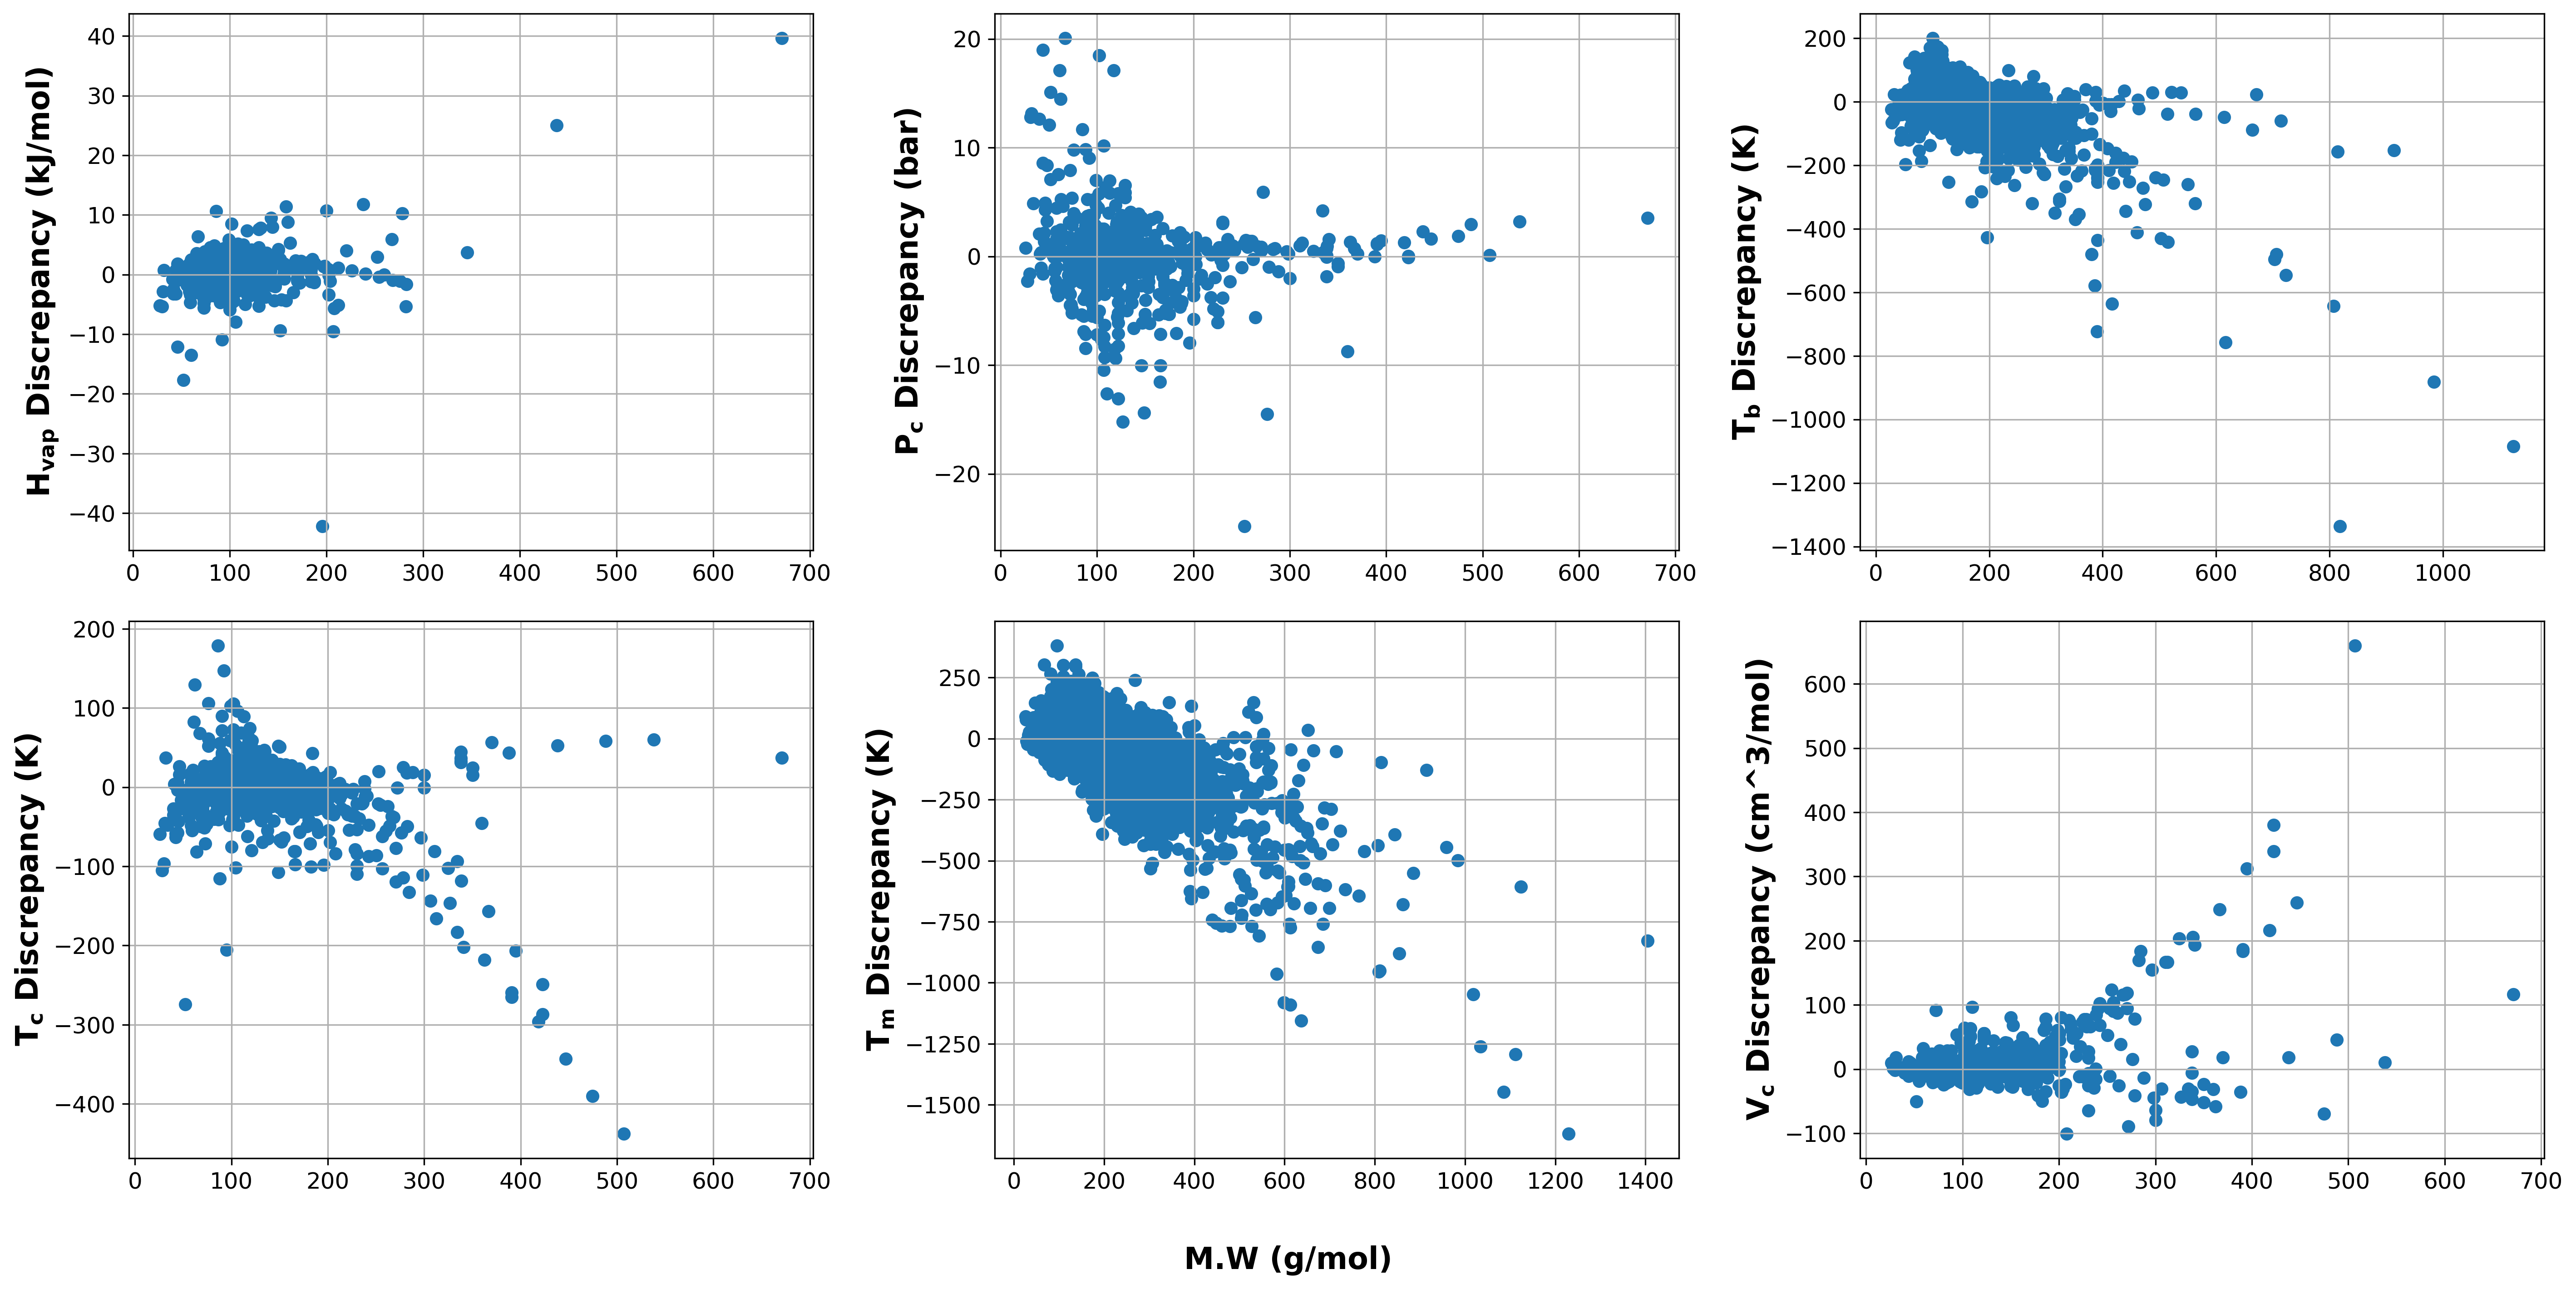
\includegraphics[width=\textwidth]{"./MW_vs_Disc.png"} %Add 6 figure 2D plots of GP Data
    \caption{Data visualization for all properties of interest. For each subplot, the x-axis is the molecular weight, the y-axis is the discrepancy between the experimental and GC predicted property value.}
    \label{fig:Data_Vis_Disc}
\end{figure}

\begin{figure}[H] %Move to SI
    \centering
    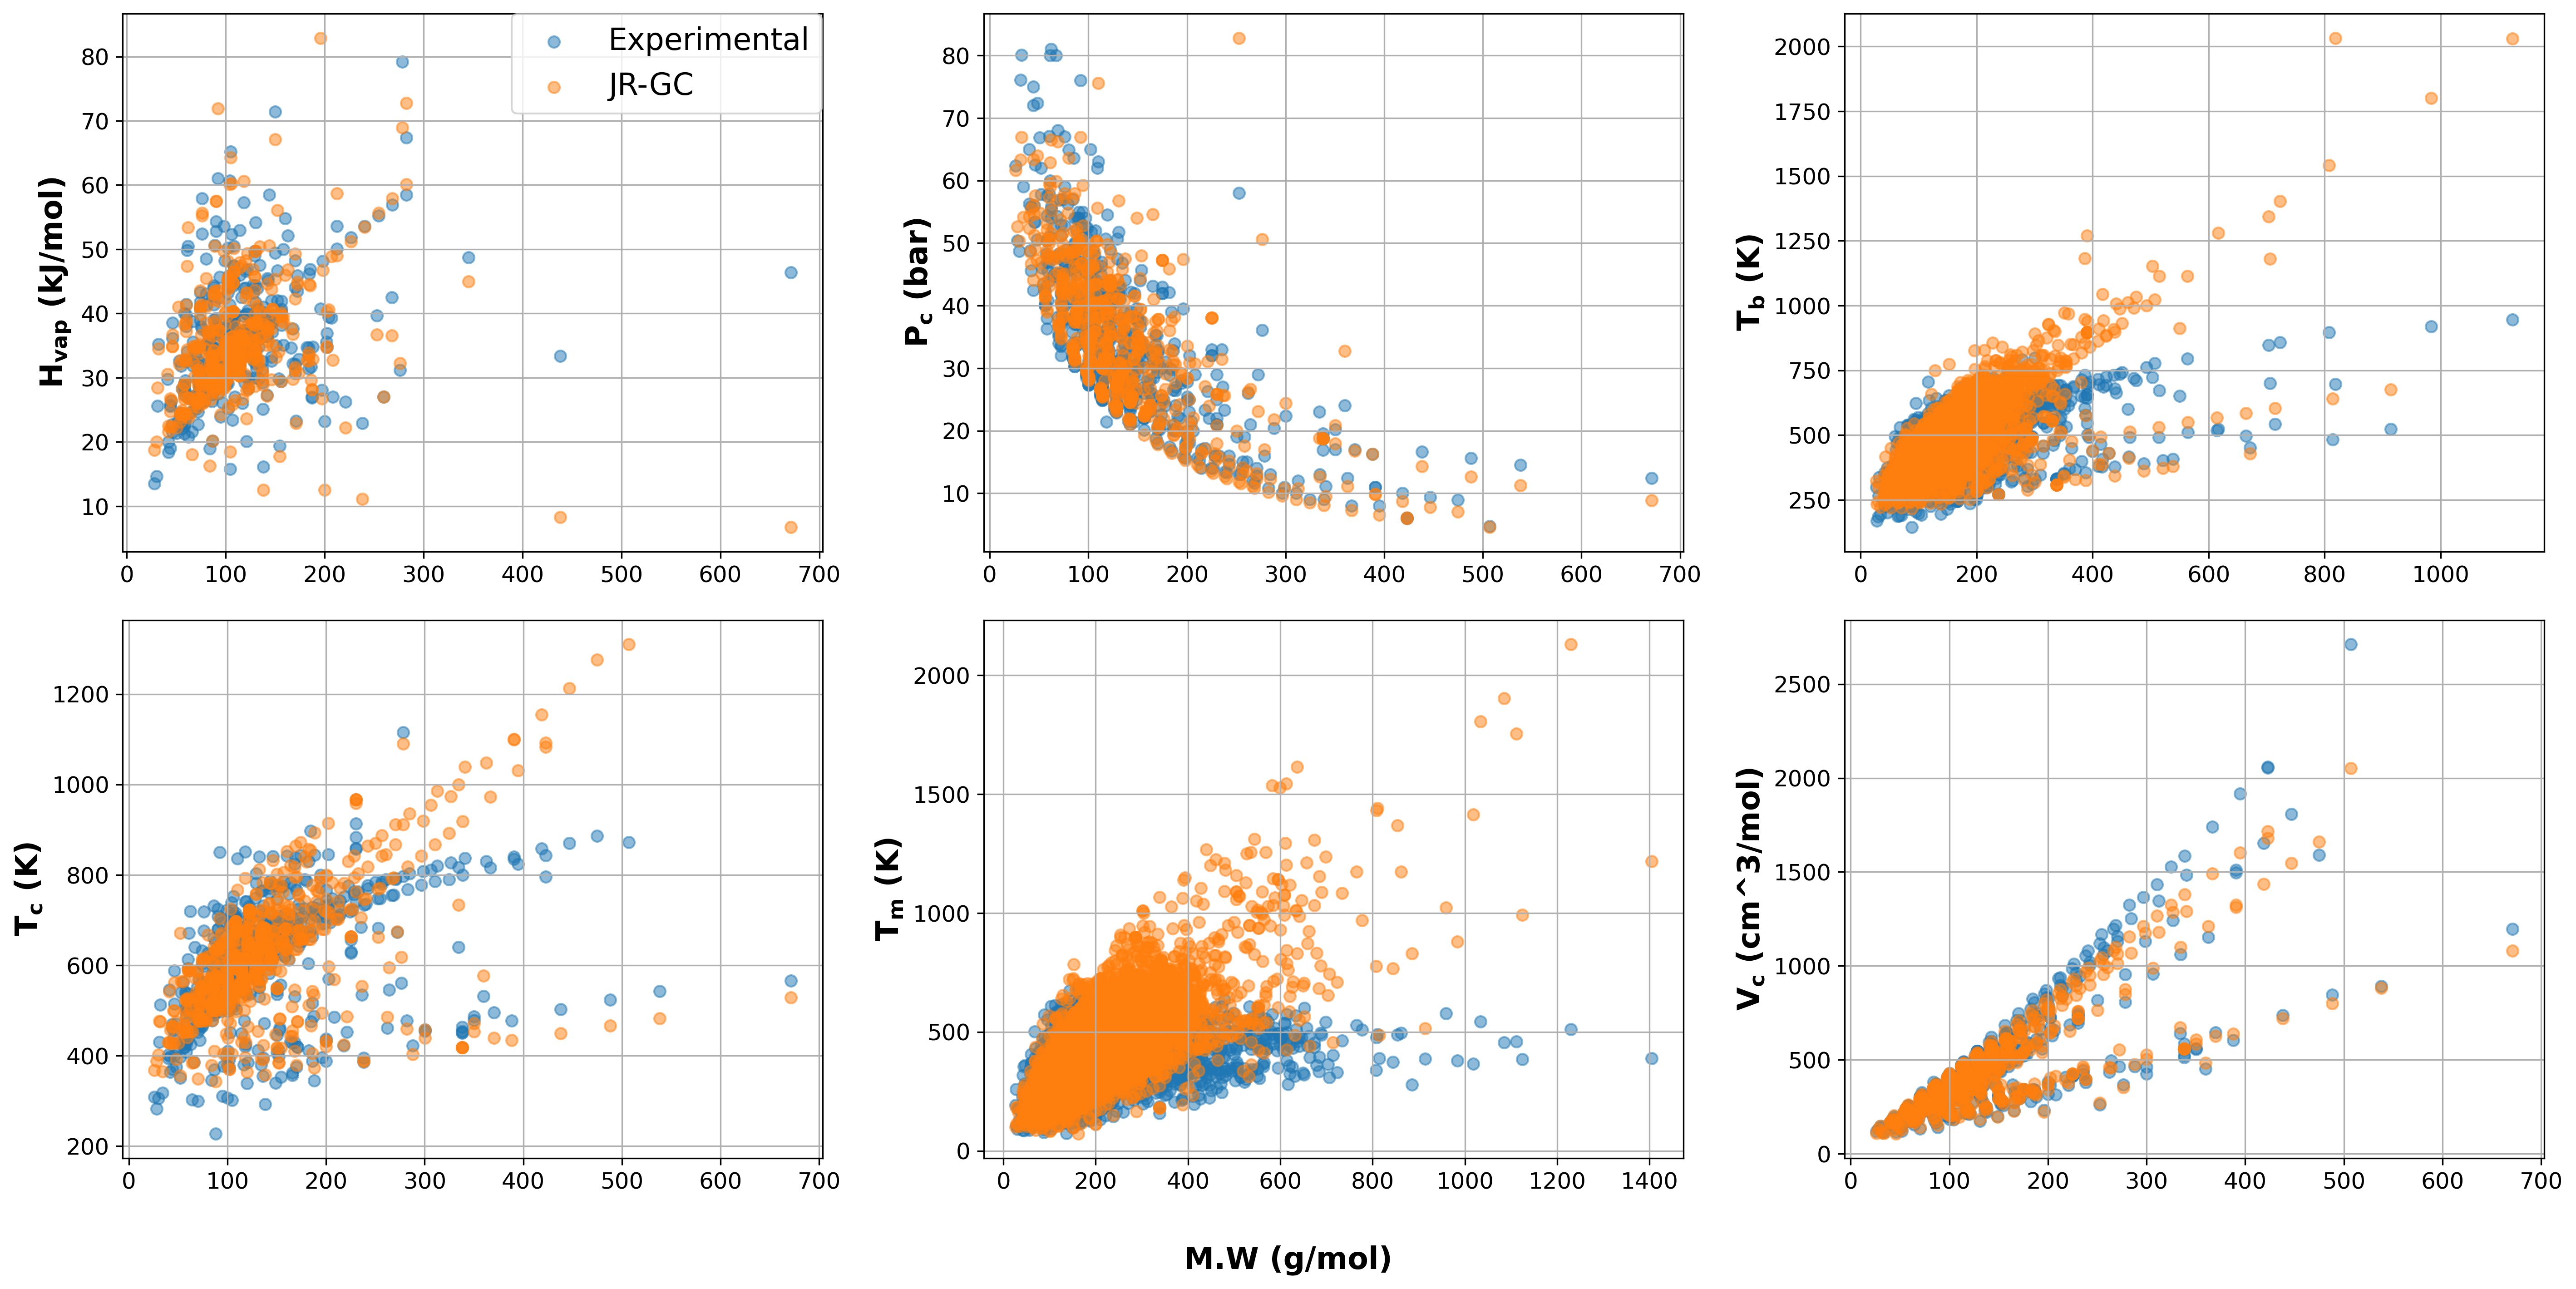
\includegraphics[width=\textwidth]{"./MW_vs_Prop.png"} %Add 6 figure 2D plots of GP Data
    \caption{Data visualization for all properties of interest. For each subplot, the x-axis is the molecular weight, the y-axis is the experimental property value (orange) or GC predicted property value (blue).}
    \label{fig:Data_Vis_Prop}
\end{figure}



\subsection{GP Modeling}
%Stratified sampling (Dinis)
When splitting data into training and testing sets, an 80/20 split was used and all features and labels were standardized to have zero mean and unit variance using the scikit-learn StandardScaler \cite{scikit-learn} . Stratified sampling was used to split the data. (Dinis to add more details). Additionally, we standardize all feature and label data by removing the mean and scaling to unit variance.

%Introduction to a kernel function and mean and variance predictions
\mcnote{GP Introduction. A short alternative to KJ's description below. Can be updated to match KJ notation and "GPs in the context of this work" if wanted}

\mcnote{To describe a Gaussian Process (GP), consider a dataset $D = \{(\xvec_i, \yexp[i]\}) \vert \xvec_i \in \mathbb{R}^d, \text{ and } \yexp[i] \in \mathbb{R}, \forall \, i \in \{1,. . ., n\}$ with inputs $\mathbf{X}$ and outputs $\yexpvec[]$. Here $\xvec$ represents the GC model predictions ($\Ygcvec$) and molecular weight ($\textbf{M.W}$) for all molecules $n$, and $\yexpvec$ represents the experimental predictions for any property $y$. If we assume that experimental data noise is independent and identically distributed with zero mean and constant variance, $\sigma_{\yexp[i]}^2$,it follows that $\yexp[i] = f(\xvec_i) + \epsilon$ where the noise is defined by $\epsilon \sim \mathcal{N}(0,\sigma_{\yexp[i]}^2)$. The GP then seeks to estimate $\yexp[i] = f(\xvec_i) + \epsilon$ as a normal distribution with mean function, $m(\xvec_i)$ for $m(\xvec_i): \mathbb{R}^d \rightarrow \mathbb{R}$, and covariance matrix, $k(\xvec_i, \xvec_i^{\prime})$ for $k: \mathbb{R}^d \times \mathbb{R}^d \rightarrow \mathbb{R}$ \cite{Frazier2018AOptimization}. We then define our GP model for all $\mathbf{X}$:
\begin{gather*}
     \yexpvec \sim \mathcal{GP} = \mathcal{N}(\boldsymbol{\mu}, \mathbf{K})
\end{gather*}

\noindent where $\boldsymbol{\mu} = (m(\xvec_1), \dots, m(\xvec_n))^\intercal$ and
\begin{gather}
    \mathbf{K}= 
    \left(
    \begin{matrix}
        k(\xvec_1,\xvec_1) & \dots & k(\xvec_1,\xvec_n) \\
        \vdots & \ddots & \vdots \\
        k(\xvec_n,\xvec_1) & \dots & k(\xvec_n,\xvec_n)
    \end{matrix}\right).
\end{gather}

We note that from a purely modeling perspective, the best accuracy will be achieved by modeling each property separately with a different GP mean function and covariance matrix given the trends in the available data. However, this requires modeling expertise and given that much of the data range for each property with regards to molecular weight has already been explored, we opt to use one general model framework which is likely to capture all properties under study in this work and any future properties of interest. In the context of using GC predictions to train a GP model, we determined that the discrepancy of the JR-GC model and experimental data is a function of molecular weight but that the relationship between the two was not always immediately obvious. However in all cases we expect that JR-GC model and the experimental property data to be linearly proportional. As such, while we use both molecular weight and JR-GC predictions as training data features, we implement a linear mean function which relies solely on the original JR-GC predictions. We fix the hyperparameters associated with the mean function such that $\boldsymbol{\mu} = \Ygcvec$.  Other model forms which were considered can be found in SI section XX. 

The covariance matrix, often called the kernel, indicates how GP features relate to each other and the smoothness of the feature. In this work, the rational quadratic (RQ) kernel is used since it accounts for varying amounts of smoothness in each dataset through hyperparameter $\alpha$. We also add a white kernel to account for uncertainty in the experimental data. The full kernel function for any two data points is defined by \eqref{kernel_final}. Mat\`ern $\frac{1}{2}$, Mat\`ern $\frac{3}{2}$, Mat\`ern $\frac{5}{2}$, and the SE kernels are examined in section \ref{sec:kern_sweep} and are defined in SI section (reference SI section).

\begin{equation}
    k(\xvec_i,\xvec_j) = \sigma_f^2 \left(1 +\frac{1}{2 \alpha} \,\mathbf{r}^\intercal \,{\ell}^{-1} \,\mathbf{r} \right)^{-\alpha} + \sigma_w^2\delta_{i,j}
    \label{kernel_final}
\end{equation}

\noindent where  $\mathbf{r} = \xvec_i - \xvec_j$, $\sigma_f^2$ is the amplitude (variance) of the process, and $\ell$ is a length scale which controls the smoothness of the function, $\sigma_w$ is the variance of the experimental noise, applied through the Kronecker delta function $\delta_{i,j}$:
\begin{gather*}
    \delta_{i,j} = 
    \begin{cases}
        0, & i\neq j,\\
        1, & i= j.
    \end{cases}
\end{gather*}

We note that hyperparameters $\alpha$, $\ell$, $\sigma_{f}$, and $\sigma_{w}$ must be inferred from the data. 

To make predictions about some new data set $\xvec^*$ we note that our training and new data follow a joint multivariate normal distribution. That is,
\begin{gather*}
    \begin{bmatrix}
        \mathbf{y} \\
        \mathbf{y}_*
    \end{bmatrix}
    \sim 
    \mathcal{N}\left(
    \begin{bmatrix}
        \boldsymbol{\mu}\\
        \boldsymbol{\mu}_*
    \end{bmatrix},
    \begin{bmatrix}
        \mathbf{K}_{nn} & \mathbf{K}_{n*} \\
        \mathbf{K}_{*n} & \mathbf{K}_{**}
    \end{bmatrix} \right).
\end{gather*}

\noindent Predictions $\mathbf{y}_*$ can then be described by the conditional distribution of the new data set given the training data set.

\begin{gather}
    \mathbf{y}_* \,|\, \xvec, \mathbf{y} \sim \mathcal{N}(\boldsymbol{\mu}_* + \mathbf{K}_{*n}\,(\mathbf{K}_{nn})^{-1}\,(\mathbf{y}-\boldsymbol{\mu}), \mathbf{K}_{**} - \mathbf{K}_{∗n} \,(\mathbf{K}_{nn})^{-1}\,\mathbf{K}_{n*}).   
\end{gather}

%General implementation details
GP models were implemented using GPflow \cite{Matthews2017GPflow:TensorFlow}. In this work, a white kernel is used to account for experimental noise and $\sigma_w$ is always trained starting from an initial value of 1.0. The hyperparameter tuning was implemented using scipy.optimize \cite{Virtanen2020SciPyPython} with the Limited-memory Broyden–Fletcher–Goldfarb–Shanno Bound (L-BFGS-B) algorithm to perform maximum likelihood estimation and was repeated ten times to avoid local hyperparameter solutions. On the first training pass, hyperparameters were all initialized at 1.0. On subsequent repeats, $\ell$, $\sigma^2_{rq}$, and $\alpha$ were uniformly selected from bounds $(0, 100]$, $(0, 1.0]$, and $(0, 100]$  respectively. Optimization bounds for $\ell$ and $\sigma^2_{rq}$ were set as $[10^{-5}, 10^2]$ and optimization bounds for $\alpha$ were set to $[10^{-5}, 5\times 10^3]$.

We use the condition number to determine the numerical stability of our models. The condition number is an indication of how small perturbations in the inputs can affect the outputs \cite{Foster2009}. As a rule of thumb, the number of significant digits lost in addition to those from machine precision is proportional to the logarithmic scaled value of a condition number \cite{NumMathComput}. Ideally, a condition number should be as close to one as possible and a condition number that is much greater than one (in this case we used 500 as a cutoff) is ill-conditioned. That is, a small change in the inputs has significant impact on the output.}

\alltodo{Do the primary authors think the reader knows what Baysian inference is? Maybe a paragraph long section before GP basics that says what it is on a high level followed by Bayes law would be helpful for vocab like likelihood, prior, evidence, etc.}
\mcnote{The readers will not know what Bayesian inference is, but I think a whole paragraph to explain these terms might not be necessary. You've done a good job of explaining them in your sections below.}
\\
\kjnote{Begin KJ proposal for explaining GPs
\subsubsection{Gaussian Process Basics}
A stochastic process is a (infinite) collection of random variables indexed by a set $\{\xvec\}$. A Gaussian process (GP) is a stochastic process where any finite number of random variables have a joint Gaussian distribution. We use $\xvec_i \in \reals^d$ to denote the index and $f: \reals^d \rightarrow \reals$ as a the random variable that is indexed by $\xvec$ (i.e., the stochastic process). A GP is specified by a mean function
\begin{gather}
    m(\xvec) := \mathbb{E}\,[f(\xvec)] \label{eq: mean}
\end{gather}
and a covariance function
\begin{gather}
    k(\xvec, \xvec') := \text{Cov}\,[f(\xvec), f(\mathbf{x'})]. \label{eq: cov}
\end{gather}
We introduce the notation 
\begin{gather*}
    f(\xvec)\sim \mathcal{GP}(m(\xvec), \, k(\xvec,\xvec'))
\end{gather*}
to denote that $f(\cdot)$ follows a GP distribution with mean function $m(\cdot)$ and covariance function $k(\cdot,\cdot)$. Equivalently, by the definition of a GP, for any finite subset $\xvec_1, \dots, \xvec_n$ of the random variables, $\mathbf{f}=(f(\xvec_1),  \dots, f(\xvec_n))^\intercal$ follows a multivariate normal distribution with a mean vector and covariance matrix governed elementwise by \eqref{eq: mean} and \eqref{eq: cov}, respectively. That is,
\begin{gather*}
     \mathbf{f} \sim \mathcal{N}(\boldsymbol{\mu}, \mathbf{K}),
\end{gather*}
where $\boldsymbol{\mu} = (m(\xvec_n), \dots, m(\xvec_n))^\intercal$ and 
\begin{gather}
    \mathbf{K} = 
    \left(
    \begin{matrix}
        k(\xvec_1,\xvec_1) & \dots & k(\xvec_1,\xvec_n) \\
        \vdots & \ddots & \vdots \\
        k(\xvec_n,\xvec_1) & \dots & k(\xvec_n,\xvec_n)
    \end{matrix}\right).
\end{gather}


In Bayesian nonparametrics, a GP is used as a prior for a random variable indexed by an infinite set. Upon observing a finite subset of these random variables, the posterior is another GP. This is commonly applied in regression settings to recover latent functions.

\subsubsection{Model Selection and Kernels}
\alltodo{other authors please confirm all kernel functions used in the models were covered here} 
\mcnote{They are}\\
When modeling with GPs, the mean and covariance functions allows the modeler to encode their (lack or) prior information on the latent function. 

In mathematics, a \texit{kernel} refers to a function that defines a similarity measure between pairs of points. In the context of GPs, a kernel is a positive-definite function that defines the covariance structure. For example, the squared exponential (SE) (i.e., Gaussian) kernel is given by
\begin{gather}
    k_{\text{SE}}(\xvec_i,\xvec_j) = \sigma_f^2 \exp \left(-\frac{1}{2}\, \mathbf{r}^\intercal \,\boldsymbol{\Lambda}^{-1} \,\mathbf{r} \right), \label{eq: sekernel}
\end{gather}
where $\mathbf{r} = \xvec_i - \xvec_j$, $\sigma_f^2$ is the amplitude (variance) of the process, and $\boldsymbol{\Lambda}$ is a matrix of length scales that control the smoothness of the function. We specify how a modeler can structure the length scale matrix to encode prior knowledge of the process at the end of this section. The SE kernel assumes the underlying function is infinitely differentiable. Thus, the SE kernel is widely used due to ability to model smooth functions \alltodo{advice needed: does this last sentence require a citation?}.

A more general form of \eqref{eq: sekernel} is the rational quadratic (RQ) kernel given by
\begin{gather}
    k_{\text{RQ}}(\xvec_i,\xvec_j) = \sigma_f^2 \left(1 +\frac{1}{2 \alpha} \,\mathbf{r}^\intercal \,\boldsymbol{\Lambda}^{-1} \,\mathbf{r} \right)^{-\alpha}. \label{eq: rationalquadkernel}
\end{gather}
The RQ kernel can model a wider range of functions by adjusting the parameter $\alpha$. In the limit $\alpha \rightarrow \infty$, it is approximately the SE kernel \eqref{eq: sekernel}. Thus, the RQ kernel is more flexible than the SE kernel. If the modeler wishes the function to exhibit variations at multiple length scales, the RQ kernel is more suitable than the SE kernel.

Finally, we review the Mat\'ern kernel governed by
\begin{gather}
    k_{\text{Mat\'ern}}(\xvec_i,\xvec_j) = \sigma_f^2 \,\frac{2^{1-\nu}}{\Gamma(\nu)} \, \left(\sqrt{2\nu} \, \mathbf{r}^\intercal \,\boldsymbol{\Lambda}^{-1} \,\mathbf{r} \right)^{\nu}\, K_\nu  \left(\sqrt{2\nu} \, \mathbf{r}^\intercal \,\boldsymbol{\Lambda}^{-1} \,\mathbf{r} \right). \label{eq: maternkern}
\end{gather}
Here, $\nu$ is a smoothness parameter, $\Gamma(\cdot)$ is the Gamma function, and $K_\nu(\cdot)$ is the modified Bessel function of the second kind. Like the RQ kernel \eqref{eq: rationalquadkernel}, Matérn kernels are a generalization of the SE kernel. It can be shown that in the limit $\nu \rightarrow \infty$, the Mat\'ern kernel becomes the SE kernel. Moreover, the SE kernel assumes infinitely differentiable (smooth) functions, while the Matérn kernel allows for varying degrees of smoothness through $\nu$. These kernels can be useful when modeling real-world phenomena with unknown or varying smoothness, providing more flexibility. Common choices for $\nu$ in machine learning and GP regresison applications literature include 3/2 and 5/2 \alltodo{GP modeling authors: please include the citations here that motivated the decision to include these kernels}. 

In principled inference, the structure of of the length scale matrix $\boldsymbol{\Lambda}$ is used to model (lack of) prior information about the function. In an isotropic GP, a single length scale is used for all input dimensions. Mathematically, this means the length scale matrix is written as $\boldsymbol{\Lambda} = \lambda^2 \, \mathbf{I}$. This modeling choice enforces that all input dimensions are equally important and have the same effect on the output. Alternatively, if one wanted to use separate length scales for each input dimension, one could elect to use an anisotropic kernel function with automatic relevance detection. This allows the kernel to capture the varying relevance of different dimensions, meaning some dimensions can be more influential than others in predicting the output. Mathematically, this means the length scale matrix is written as $\boldsymbol{\Lambda} = \text{diag}(\lambda_1^2,\dots,\lambda_d^2)$.

In this section, we covered stationary kernel functions that are common in application literature for GPs \alltodo{citation needed?}. For a more generalized perspective on classes of kernel functions, we refer the interested reader to \citeauthor{Genton} \cite{Genton}.

\subsubsection{Gaussian Processes for Regression}
Consider the regression setting where we are supplied with a dataset $\mathcal{D} = \{(\xvec_i, y_i)\}_{i=1}^n$ composed of $n$ pairs of regressors $\xvec_i \in \reals^d$ and observations $y_i \in \reals$. The objective is to recover the latent data generating process $f(\cdot)$. In most practical settings, the underlying process is perturbed by noise $\varepsilon_i$. That is,
\begin{gather*}
    y_i = f(\xvec_i) + \varepsilon_i, \quad i \in \{1,\dots, n\},
\end{gather*}
where $\varepsilon_i \stackrel{\text{i.i.d.}}{\sim} \mathcal{N}(0,\sigma^2)$. In GP regression (GPR), it is assumed that $f(\cdot)\sim \mathcal{GP}(m(\cdot),k(\cdot,\cdot))$. This assumption is called the prior. By linearity of expectation,
\begin{gather*}
    \mathbb{E}\,[y_i\,|\,\xvec_i] = m(\xvec_i)
\end{gather*}
and
\begin{gather*}
    \text{Cov}\,[y_i\, | \,\xvec_i, y_j \, | \,\xvec_j] = k(\xvec_i, \xvec_j) + \sigma^2 \,\delta_{i,j},
\end{gather*}
where $\delta_{i,j}$ is the Kronecker delta function
\begin{gather*}
    \delta_{i,j} = 
    \begin{cases}
        0, & i\neq j,\\
        1, & i= j.
    \end{cases}
\end{gather*}
The goal in the regression setting is to predict $f(\cdot)$ over a test set $\xvec^*$. By the GP prior on $f(\cdot)$, the finite set of training and test outputs follow a joint multivariate normal distribution. That is,
\begin{gather*}
    \begin{bmatrix}
        \mathbf{y} \\
        \mathbf{f}_*
    \end{bmatrix}
    \sim 
    \mathcal{N}\left(
    \begin{bmatrix}
        \boldsymbol{\mu}\\
        \boldsymbol{\mu}_*
    \end{bmatrix},
    \begin{bmatrix}
        \mathbf{K}_{nn} +\sigma^2\,\mathbf{I} & \mathbf{K}_{n*} \\
        \mathbf{K}_{*n} & \mathbf{K}_{**}
    \end{bmatrix} \right).
\end{gather*}
Here, $\mathbf{K}_{nn}$ is the $n\times n$ covariance matrix defined on the training data,  $\mathbf{K}_{n*}$ is the $n \times |\text{test}|$ covariance matrix, etc. 

\kjtodo{Left off here} To make predictions at new test points $\xvec_*$, one computes the conditional distribution of the test outputs given the training data $\mathbf{f}_* \,|\, \xvec, \mathbf{y}$. This is done by computing the finite-dimensional conditional distribution
\begin{gather}
    \mathbf{f}_* \,|\, \xvec, \mathbf{y} \sim \mathcal{N}(\boldsymbol{\mu}_* + \mathbf{K}_{*n}\,(\mathbf{K}_{nn} +\sigma^2\,\mathbf{I})^{-1}\,(\mathbf{y}-\boldsymbol{\mu}), \mathbf{K}_{**} - \mathbf{K}_{∗n} \,(\mathbf{K}_{nn}+\sigma^2\,\mathbf{I})^{-1}\,\mathbf{K}_{n*}).   
\end{gather}

\subsection{GPs in the context of this work}
In this work, we define $\mathcal{D} = \{(\Ygc[i], \text{M.W}_i), \yexp[i])\}_{i=1}^n$ for all molecules $n$ and any property of interest $y \in [H_{vap}, P_c, T_c, T_b ,T_M, V_c]$. We define $\Ygc[i] \text{ } \forall \text{ } i\in n$ as JR-GC model predictions, $\text{M.W}_i \text{ } \forall \text{ } i\in n$ as the molecular weights, and $\yexp[i] \text{ } \forall \text{ } i\in n$ as the experimental values. We begin by noting that from a modeling perspective, the best accuracy will be achieved by analyzing trends in the available data and setting the GP mean and covariance functions to capture those trends. However, this requires modeling expertise and given that much of the data range for each property with regards to molecular weight has already been explored, we opt to use one general model framework which is likely to capture all properties under study in this work and any future properties of interest. The effect of model form on our results is examined in section \ref{sec:kern_sweep}.

We determined in section XX that the discrepancy of the JR-GC model for each property of interest and experimental property data is a function of molecular weight but that the relationship between the two was not always immediately obvious. However in all cases we expect that JR-GC model and the experimental property data to be linearly proportional. As such, while we use both molecular weight and JR-GC predictions as training data features, we implement a linear mean function which relies solely on the original JR GC predictions. We fix the hyperparameters associated with the mean function such that $m(\xvec) = \Ygcvec$ where $\Ygc[i] \text{ } \forall \text{ } i\in n$ are the JR-GC model predictions for $n$ molecules and any property of interest $y$. This mean function is especially appropriate when the JR-GC models faithfully represent the trend of experimental data. Other model forms which were considered can be found in SI section XX. We choose the rational quadratic (RQ) kernel as the base kernel function for the GP models of every property to account for varying levels of smoothness. We add a white kernel with variance $\sigma_w$ to the RQ kernel to account for uncertainty in the experimental data such that the final covariance function used in this work is defined by \eqref{kernel_final}. 

\begin{equation}
    k(\xvec_i,\xvec_j) = \sigma_f^2 \left(1 +\frac{1}{2 \alpha} \,\mathbf{r}^\intercal \,\boldsymbol{\Lambda}^{-1} \,\mathbf{r} \right)^{-\alpha} + \sigma_w^2\delta_{i,j} 
    \label{kernel_final}
\end{equation} 

GP models were implemented using GPflow \cite{Matthews2017GPflow:TensorFlow}. The hyperparameter tuning was implemented using scipy.optimize \cite{Virtanen2020SciPyPython} with the Limited-memory Broyden–Fletcher–Goldfarb–Shanno Bound (L-BFGS-B) algorithm to perform maximum likelihood estimation and was repeated ten times to avoid local hyperparameter solutions. On the first training pass, hyperparameters were all initialized at 1.0. On subsequent repeats, $\ell$ and $\alpha$ were uniformly selected from bounds $(0, 100]$ and $(0, 100]$ respectively. $\sigma^2_f$ was selected from a log-normal distribution with bounds $[0,1.0]$ and $\sigma_w$ was always initialized at $1.0$. A more nuanced method would be to initialize $\sigma_w$ as the scaled experimental uncertainty when available. Optimization bounds for $\alpha$ were set to $[10^{-5}, 10^2]$ and all other hyperparameters were optimized within bounds $[10^{-5}, 5\times 10^3]$.

We use the condition number to determine the numerical stability of our models. The condition number is an indication of how small perturbations in the inputs can affect the outputs \cite{Foster2009}. As a rule of thumb, the number of significant digits lost in addition to those from machine precision is proportional to the logarithmic scaled value of a condition number \cite{NumMathComput}. Ideally, a condition number should be as close to one as possible and a condition number that is much greater than one (in this case we used 500 as a cutoff) is ill-conditioned. That is, a small change in the inputs has significant impact on the output.

\subsubsection{Hyperparameter Estimation and Criteria for Model Selection}
As shown in the kernel section \kjtodo{reference later}, the behavior of mean and kernel functions are somewhat dictated by their parameters $\boldsymbol{\theta}$ \kjtodo{retype with theta subscript}. If these are not chosen by the practitioner, they must be inferred from data. Furthermore, one might be interested in comparing the performance of several GP models and selecting the best performing model (i.e., model selection). The evidence (i.e., marginal likelihood) allows us to accomplish both.

The evidence is given by
\begin{gather}
    p(\mathbf{y}\, | \, \xvec) = \int p(\mathbf{y}\, | \, \mathbf{f}) \,  p(\mathbf{f}\, | \, \xvec) \, \text{d}\mathbf{f},
\end{gather}
where we marginalize over the the function values $\mathbf{f}$. Given that both $p(\mathbf{y}\, | \, \mathbf{f})$ and $ p(\mathbf{f}\, | \, \mathbf{X})$ are Gaussian, the marginal likelihood can be computed in closed form. Moreover, the marginal likelihood has distribution,
\begin{gather}
    \mathbf{y}\, | \, \mathbf{X} \sim \mathcal{N}(\boldsymbol{\mu}, \mathbf{K}_{nn} + \sigma^2 \,\mathbf{I}),
\end{gather}
or
\begin{gather}
    p(\mathbf{y}\, | \, \mathbf{X}) = (2\pi)^{-n/2}\,\text{det}(\mathbf{K}_{nn} + \sigma^2 \,\mathbf{I})^{-1}\,\exp \left( -\frac{1}{2}(\mathbf{y}-\boldsymbol{\mu})^\intercal \, (\mathbf{K}_{nn} + \sigma^2 \,\mathbf{I})^{-1}\,(\mathbf{y}-\boldsymbol{\mu})\right)
\end{gather}
}

\subsection{Hybrid Modeling}
\alltodo{Feel free to move this section wherever it fits best}\\

\kjnote{\\
In their seminal work, statisticians \kjtodo{cite KOH} developed a framework for Bayesian calibration of computer models, which has become commonplace in the physical sciences. \kjtodo{write review about this}\\

Given $n$ observations $\mathbf{y}=(y_1,\dots,y_n)^\intercal$ generated by manipulating a controlled variable $\xvec_i = (x_{i,1},\dots,x_{i,d})^\intercal$, the goal of model calibration is to find the underlying mapping $\zeta: \mathbb{R}^d \rightarrow \mathbb{R}$ that describes the physical scenario. This relationship is written as
\begin{gather}
    y_i = \zeta(\mathbf{x}_i) + \varepsilon_i, \quad i = 1,\dots,n. \label{eq: trueprocess}
\end{gather}

In practice, $\zeta(\cdot)$ is unknown, and we rely on a simulation or lower-fidelity model denoted $\eta(\mathbf{x}, \boldsymbol{\theta})$. The model has parameters $\boldsymbol{\theta}=(\theta_1,\dots,\theta_p)^\intercal$ that need to be estimated from data. To account for discrepancy in the model $\eta(\cdot,\cdot)$, a model discrepancy function $\delta: \mathbb{R}^d \rightarrow \mathbb{R}$ is included. This leads to:
\begin{gather}
     y_i = \zeta(\mathbf{x}_i) + \varepsilon_i = \eta(\mathbf{x}_i,\boldsymbol{\theta}) + \delta(\mathbf{x}_i) + \varepsilon_i, \quad i = 1,\dots,n.
\end{gather}

Typically, $\delta(\cdot)$ is modeled using a Gaussian Process (GP), although any nonparametric method can be used in practice. If $\eta(\cdot,\cdot)$ is computationally expensive, it can also be represented as a GP. In this work, we assume that $\eta(\cdot,\cdot)$ can be modeled directly and $\delta(\cdot)\sim \mathcal{GP}(m(\cdot),k(\cdot,\cdot))$. Thus, the hybrid model reduces to the GP
\begin{gather}
    \zeta(\mathbf{x}) \sim \mathcal{GP}(\eta(\mathbf{x},\boldsymbol{\theta}) + m(\mathbf{x}), k(\mathbf{x}, \mathbf{x}'))
\end{gather}

In this application, we do not have parameters $\boldsymbol{\theta}$ to estimate in the low-fidelity model. Moreover, estimation of $\zeta(\cdot)$ is accomplished by estimating the parameters in the GP mean and covariance functions.
\alltodo{please confirm Jobac model has no parameters that are being fit}.
}


\subsection{Error Metrics}
\alltodo{Do we need both MAPE and MAPD? Should we change "deviation" to "error"?.}
\mcnote{We don't. We currently use both now, but it's up to Barnabas to decide the final metrics so I wrote down both for now.}
We use mean absolute error (MAE), mean absolute prediction error (MAPE), mean absolute percent deviation (MAPD), coefficient of determination ($R^2$), and root mean squared error (RMSE) to quantify and critically analyze the error of our GP models. This section gives an overview of the definition of these error metrics. Note that in \eqref{eq:COD}, $\overline{y_{\text{exp}}}$ is the average value of $\mathbf{y}_{\text{exp}}$. 

\begin{equation}
    \text{MAE} = \frac{1}{N} \sum_{i=1}^{N} \left| y_{\text{exp}_i} - \mu(\mathbf{x}_i) \right|
    \label{eq:MAE}
\end{equation}

\begin{equation}
    \alltodo{\text{MAPE}} = \frac{1}{N} \sum_{i=1}^{N} \left| \frac{y_{\text{exp}_i} - \mu(\mathbf{x}_i)}{y_{\text{exp}_i}} \right|
    \label{eq:MAPE}
\end{equation}

\begin{equation}
    \text{MAP\alltodo{D}} = \frac{1}{N} \sum_{i=1}^{N} \left| \frac{y_{\text{exp}_i} - \mu(\mathbf{x}_i)}{y_{\text{exp}_i}} \right| \times 100\%
    \label{eq:MAPD}
\end{equation}

\begin{equation}
    R^2 = 1 - \frac{\sum_{i=1}^{N} \left( y_{\text{exp}_i} - \mu(\mathbf{x}_i) \right)^2}{\sum_{i=1}^{N} \left( y_{\text{exp}_i} - \overline{y_{\text{exp}}} \right)^2}
    \label{eq:COD}
\end{equation}

\begin{equation}
    \text{RMSE} = \sqrt{\frac{1}{N} \sum_{i=1}^{N} \left( y_{\text{exp}_i} - \mu(\mathbf{x}_i) \right)^2}
    \label{eq:RMSE}
\end{equation}

\section{Results and Discussion}


\subsection{Kernel Sweep} 
\label{sec:kern_sweep}
%Note this will be replaced with a table for each property and prediction and the "best" kernel with all others in the SI

\begin{table}[H]
    \centering
    \begin{tabular}{>{\centering\arraybackslash}p{1.0cm}>{\centering\arraybackslash}p{1.0cm}>{\centering\arraybackslash}p{0.75cm}>{\centering\arraybackslash}p{0.75cm}>{\centering\arraybackslash}p{1.0cm}>{\centering\arraybackslash}p{1.0cm}>{\centering\arraybackslash}p{0.75cm}>{\centering\arraybackslash}p{0.75cm}>{\centering\arraybackslash}p{1cm}>{\centering\arraybackslash}p{0.75cm}>{\centering\arraybackslash}p{0.75cm}>{\centering\arraybackslash}p{0.75cm}>{\centering\arraybackslash}p{1cm}>{\centering\arraybackslash}p{0.75cm}}
       \vspace{1.15cm}  kern ID& 
       \vspace{1.15cm} Cond   N& 
       \vspace{0.66cm} R2  train     1&  
 \vspace{0.66cm} R2  test   1& 
 \vspace{0.146cm} (\%) MAPD test \hspace{0.5cm}  1&  
 ($kJ \cdot mol^{-1}$) MAE test  \hspace{0.5cm}   1&  \vspace{0.66cm} R2 train   4& 
 \vspace{0.66cm} R2 test   4& 
 \vspace{0.146cm} (\%) MAPD test  \hspace{0.5cm}  4&  
 ($kJ \cdot mol^{-1}$) MAE test  \hspace{0.5cm}   4& \vspace{0.66cm} R2   train      5& 
 \vspace{0.66cm} R2   test     5& 
 \vspace{0.146cm} (\%) MAPD test  \hspace{0.5cm}   5&
 ($kJ \cdot mol^{-1}$) MAE test  \hspace{0.5cm}   5
 
%\\ 

\\
          rbf(2)   &  221.3&  0.86&  0.9&  5.14&  1.75&  0.86&  0.91&  5.1&  1.73& 0.86& 0.91& 5.13&1.74
\\
         rq(2)   &  244.34&  0.86&  0.9&  5.15&  1.76&  0.86&  0.9&  5.11&  1.74& 0.86& 0.91& 5.13&1.74
\\
         mt1(2) &  155&  0.9&  0.89&  5.53&  1.9&  0.9&  0.89&  5.57&  1.91& 0.89& 0.9& 5.49&1.88
\\
         mt3(2)&  193.68&  0.86&  0.9&  5.21&  1.79&  0.86&  0.9&  5.18&  1.77& 0.86& 0.9& 5.19&1.77
\\
         mt5(2) &  204.09&  0.86&  0.9&  5.18&  1.77&  0.86&  0.9&  5.14&  1.75& 0.86& 0.9& 5.16&1.76
\\
         rbf    &  221.3&  0.85&  0.88&  5.23&  1.84&  0.85&  0.88&  5.11&  1.8& 0.86& 0.88& 5.36&1.89
\\
         rq   &  244.34&  0.86&  0.88&  5.34&  1.87&  0.86&  0.88&  5.28&  1.86& 0.86& 0.88& 5.34&1.88
\\
         mt1  &  155&  0.91&  0.87&  5.42&  1.9&  0.91&  0.87&  5.39&  1.89& 0.9& 0.87& 5.36&1.88
\\
         mt3  &  193.68&  0.86&  0.88&  5.29&  1.85&  0.86&  0.88&  5.23&  1.84& 0.86& 0.88& 5.29&1.86
\\
 mt5  & 204.09& 0.86& 0.88& 5.28& 1.85& 0.85& 0.88& 5.18& 1.83& 0.86& 0.88& 5.31&1.87
\\
    \end{tabular}
    \caption{Kernel Sweep Summary for $\Delta H_{vap}$ using models 1, 4, and 5}
    \label{tab:hvap_ksweep}
\end{table}


\vspace{0.5cm}


\begin{table}[H]
    \centering
    \begin{tabular}{>{\centering\arraybackslash}p{1.0cm}>{\centering\arraybackslash}p{1.0cm}>{\centering\arraybackslash}p{0.75cm}>{\centering\arraybackslash}p{0.75cm}>{\centering\arraybackslash}p{1.0cm}>{\centering\arraybackslash}p{1.0cm}>{\centering\arraybackslash}p{0.75cm}>{\centering\arraybackslash}p{0.75cm}>{\centering\arraybackslash}p{1cm}>{\centering\arraybackslash}p{0.75cm}>{\centering\arraybackslash}p{0.75cm}>{\centering\arraybackslash}p{0.75cm}>{\centering\arraybackslash}p{1cm}>{\centering\arraybackslash}p{0.75cm}}
    \vspace{1.15cm}  kern ID& 
    \vspace{1.15cm} Cond   N& 
    \vspace{0.66cm} R2  train     1&  
    \vspace{0.66cm} R2  test   1& 
    \vspace{0.146cm} (\%) MAPD test \hspace{0.5cm}  1&  
 \vspace{0.146cm} (K) MAE test  \hspace{0.5cm}   1&  \vspace{0.66cm} R2 train   4& \vspace{0.66cm} R2 test   4& \vspace{0.146cm} (\%) MAPD test  \hspace{0.5cm}  4&
 \vspace{0.146cm} (K) MAE test  \hspace{0.5cm}   4&
 \vspace{0.66cm} R2   train      5&
 \vspace{0.66cm} R2   test     5&
 \vspace{0.146cm} (\%) MAPD test  \hspace{0.5cm}   5&
 \vspace{0.146cm} (K) MAE test  \hspace{0.5cm}   5
 
%\\ 

\\
          rbf(2)   &  320.59&  0.94&  0.93&  3.87&  20.96&  0.94&  0.93&  3.83&  20.72& 0.95& 0.93& 3.91&20.95
\\
         rq(2)   &  354.16&  0.95&  0.93&  3.89&  20.92&  0.95&  0.93&  3.88&  20.92& 0.95& 0.93& 3.9&20.95
\\
         mt1(2) &  225.2&  0.98&  0.93&  3.96&  21.29&  0.98&  0.93&  3.93&  21.19& 0.98& 0.93& 3.94&21.19
\\
         mt3(2)&  281.35&  0.96&  0.93&  3.9&  20.97&  0.96&  0.93&  3.89&  20.93& 0.96& 0.93& 3.91&21.04
\\
         mt5(2) &  296.29&  0.95&  0.93&  3.89&  20.86&  0.95&  0.93&  3.87&  20.77& 0.96& 0.93& 3.9&20.96
\\
         rbf    &  320.59&  0.94&  0.93&  3.87&  21.03&  0.94&  0.93&  3.83&  20.73& 0.95& 0.93& 3.92&20.96
\\
         rq   &  354.16&  0.95&  0.93&  3.9&  20.94&  0.95&  0.93&  3.89&  20.95& 0.95& 0.93& 3.9&20.97
\\
         mt1  &  225.2&  0.98&  0.93&  3.96&  21.23&  0.98&  0.93&  3.93&  21.19& 0.98& 0.93& 3.94&21.2
\\
         mt3  &  281.35&  0.96&  0.93&  3.91&  21.01&  0.96&  0.93&  3.9&  20.96& 0.96& 0.93& 3.92&21.06
\\
 mt5  & 296.29& 0.95& 0.93& 3.89& 20.88& 0.95& 0.93& 3.87& 20.8& 0.95& 0.93& 3.91&20.97
\\
    \end{tabular}
    \caption{Kernel Sweep Summary for $T_{c}$ using models 1, 4, and 5}
    \label{tab:tc_ksweep}
\end{table}



\vspace{0.5cm}



\begin{table}[H]
    \centering
    \begin{tabular}{>{\centering\arraybackslash}p{1.0cm}>{\centering\arraybackslash}p{1.0cm}>{\centering\arraybackslash}p{0.75cm}>{\centering\arraybackslash}p{0.75cm}>{\centering\arraybackslash}p{1.0cm}>{\centering\arraybackslash}p{1.0cm}>{\centering\arraybackslash}p{0.75cm}>{\centering\arraybackslash}p{0.75cm}>{\centering\arraybackslash}p{1cm}>{\centering\arraybackslash}p{0.75cm}>{\centering\arraybackslash}p{0.75cm}>{\centering\arraybackslash}p{0.75cm}>{\centering\arraybackslash}p{1cm}>{\centering\arraybackslash}p{0.75cm}}
    \vspace{1.15cm}  kern ID& 
    \vspace{1.15cm} Cond   N& 
    \vspace{0.66cm} R2  train     1&  
    \vspace{0.66cm} R2  test   1& 
    \vspace{0.146cm} (\%) MAPD test \hspace{0.5cm}  1&  
 \vspace{0.146cm} (Bars) MAE test  \hspace{0.5cm}   1&  \vspace{0.66cm} R2 train   4& \vspace{0.66cm} R2 test   4& \vspace{0.146cm} (\%) MAPD test  \hspace{0.5cm}  4&
 \vspace{0.146cm} (Bars) MAE test  \hspace{0.5cm}   4&
 \vspace{0.66cm} R2   train      5&
 \vspace{0.66cm} R2   test     5&
 \vspace{0.146cm} (\%) MAPD test  \hspace{0.5cm}   5&
 \vspace{0.146cm} (Bars) MAE test  \hspace{0.5cm}   5
 
%\\ 

\\
          rbf(2)   &  288.35&  0.94&  0.94&  5.35&  1.91&  0.94&  0.94&  5.41&  1.93& 0.94& 0.94& 5.47&1.94
\\
         rq(2)   &  324.91&  0.94&  0.93&  5.39&  1.92&  0.94&  0.94&  5.41&  1.93& 0.94& 0.94& 5.47&1.94
\\
         mt1(2) &  201.31&  0.96&  0.93&  5.57&  1.94&  0.96&  0.94&  5.48&  1.92& 0.96& 0.94& 5.56&1.93
\\
         mt3(2)&  251.63&  0.94&  0.93&  5.47&  1.95&  0.94&  0.94&  5.42&  1.92& 0.94& 0.93& 5.44&1.93
\\
         mt5(2) &  265.37&  0.94&  0.93&  5.45&  1.95&  0.94&  0.94&  5.4&  1.92& 0.94& 0.94& 5.42&1.92
\\
         rbf    &  288.35&  0.94&  0.94&  5.44&  1.93&  0.94&  0.94&  5.36&  1.92& 0.94& 0.94& 5.38&1.92
\\
         rq   &  324.91&  0.94&  0.94&  5.4&  1.92&  0.94&  0.94&  5.36&  1.92& 0.94& 0.94& 5.38&1.92
\\
         mt1  &  201.31&  0.96&  0.93&  5.57&  1.94&  0.95&  0.93&  5.44&  1.92& 0.95& 0.93& 5.5&1.92
\\
         mt3  &  251.63&  0.94&  0.94&  5.44&  1.93&  0.94&  0.94&  5.41&  1.93& 0.94& 0.94& 5.44&1.93
\\
 mt5  & 265.37& 0.94& 0.94& 5.39& 1.92& 0.94& 0.94& 5.36& 1.92& 0.94& 0.94& 5.4&1.92
\\
    \end{tabular}
    \caption{Kernel Sweep Summary for $P_{c}$ using models 1, 4, and 5}
    \label{tab:pc_ksweep}
\end{table}

\vspace{0.5cm}


\begin{table}[H]
    \centering
    \begin{tabular}{>{\centering\arraybackslash}p{1.0cm}>{\centering\arraybackslash}p{1.0cm}>{\centering\arraybackslash}p{0.75cm}>{\centering\arraybackslash}p{0.75cm}>{\centering\arraybackslash}p{1.0cm}>{\centering\arraybackslash}p{1.0cm}>{\centering\arraybackslash}p{0.75cm}>{\centering\arraybackslash}p{0.75cm}>{\centering\arraybackslash}p{1cm}>{\centering\arraybackslash}p{0.75cm}>{\centering\arraybackslash}p{0.75cm}>{\centering\arraybackslash}p{0.75cm}>{\centering\arraybackslash}p{1cm}>{\centering\arraybackslash}p{0.75cm}}
       \vspace{1.15cm}  kern ID& 
       \vspace{1.15cm} Cond   N& 
       \vspace{0.66cm} R2  train     1&  
 \vspace{0.66cm} R2  test   1& 
 \vspace{0.146cm} (\%) MAPD test \hspace{0.5cm}  1&  
 ($cm^{3} \cdot mol^{-1}$) MAE test  \hspace{0.5cm}   1&  \vspace{0.66cm} R2 train   4& \vspace{0.66cm} R2 test   4& \vspace{0.146cm} (\%) MAPD test  \hspace{0.5cm}  4&  
 ($cm^{3} \cdot mol^{-1}$) MAE test  \hspace{0.5cm}   4& \vspace{0.66cm} R2   train      5& 
 \vspace{0.66cm} R2   test     5& 
 \vspace{0.146cm} (\%) MAPD test  \hspace{0.5cm}   5&
 ($cm^{3} \cdot mol^{-1}$) MAE test  \hspace{0.5cm}   5
 
%\\ 

\\
          rbf(2)   &  341.77&  0.99&  0.98&  3.66&  17.84&  0.99&  0.98&  3.59&  16.74& 0.99& 0.98& 3.62&16.83
\\
         rq(2)   &  368.58&  0.99&  0.98&  3.64&  17.13&  0.99&  0.98&  3.58&  16.82& 0.99& 0.98& 3.6&16.94
\\
         mt1(2) &  243.1&  1&  0.98&  3.4&  16.59&  1&  0.98&  3.26&  16.15& 1& 0.98& 3.24&15.92
\\
         mt3(2)&  302.36&  1&  0.96&  3.64&  19.73&  0.99&  0.98&  3.61&  17.17& 0.99& 0.98& 3.59&17.04
\\
         mt5(2) &  317.61&  0.99&  0.98&  3.73&  18.16&  0.99&  0.98&  3.61&  17.14& 0.99& 0.98& 3.6&16.99
\\
         rbf    &  341.77&  0.99&  0.96&  3.95&  20.24&  0.99&  0.98&  3.58&  16.68& 0.99& 0.98& 3.61&16.79
\\
         rq   &  368.58&  0.99&  0.98&  3.66&  17.64&  0.99&  0.98&  3.59&  16.73& 0.99& 0.98& 3.61&16.82
\\
         mt1  &  243.1&  1&  0.98&  3.38&  16.84&  1&  0.98&  3.3&  16.18& 1& 0.98& 3.28&15.97
\\
         mt3  &  302.36&  0.99&  0.98&  3.63&  17.23&  0.99&  0.98&  3.6&  17.11& 0.99& 0.98& 3.57&16.95
\\
 mt5  & 317.61& 0.99& 0.98& 3.73& 18.24& 0.99& 0.98& 3.61& 17.12& 0.99& 0.98& 3.6&16.9
\\
    \end{tabular}
    \caption{Kernel Sweep Summary for $V_{c}$ using models 1, 4, and 5}
    \label{tab:vc_ksweep}
\end{table}


\vspace{0.5cm}



\begin{table}[H]
    \centering
    \begin{tabular}{>{\centering\arraybackslash}p{1.0cm}>{\centering\arraybackslash}p{1.25cm}>{\centering\arraybackslash}p{0.75cm}>{\centering\arraybackslash}p{0.75cm}>{\centering\arraybackslash}p{1.0cm}>{\centering\arraybackslash}p{1.0cm}>{\centering\arraybackslash}p{0.75cm}>{\centering\arraybackslash}p{0.75cm}>{\centering\arraybackslash}p{1cm}>{\centering\arraybackslash}p{0.75cm}>{\centering\arraybackslash}p{0.75cm}>{\centering\arraybackslash}p{0.75cm}>{\centering\arraybackslash}p{1cm}>{\centering\arraybackslash}p{0.75cm}}
    \vspace{1.15cm}  kern ID& 
    \vspace{1.15cm} Cond   N& 
    \vspace{0.66cm} R2  train     1&  
    \vspace{0.66cm} R2  test   1& 
    \vspace{0.146cm} (\%) MAPD test \hspace{0.5cm}  1&  
 \vspace{0.146cm} (K) MAE test  \hspace{0.5cm}   1&  \vspace{0.66cm} R2 train   4& \vspace{0.66cm} R2 test   4& \vspace{0.146cm} (\%) MAPD test  \hspace{0.5cm}  4&
 \vspace{0.146cm} (K) MAE test  \hspace{0.5cm}   4&
 \vspace{0.66cm} R2   train      5&
 \vspace{0.66cm} R2   test     5&
 \vspace{0.146cm} (\%) MAPD test  \hspace{0.5cm}   5&
 \vspace{0.146cm} (K) MAE test  \hspace{0.5cm}   5
 
%\\ 

\\
          rbf(2)   &  1950.81&  0.89&  0.85&  4.55&  20.57&  0.89&  0.83&  4.57&  20.78& 0.89& 0.88& 4.51&20.11
\\
         rq(2)   &  2186.64&  0.9&  0.88&  4.5&  20.21&  0.9&  0.88&  4.48&  20.11& 0.9& 0.88& 4.48&20.03
\\
         mt1(2) &  1360.19&  0.95&  0.88&  4.41&  19.73&  0.96&  0.88&  4.39&  19.57& 0.95& 0.88& 4.39&19.58
\\
         mt3(2)&  1703.21&  0.9&  0.87&  4.5&  20.27&  0.9&  0.87&  4.49&  20.26& 0.9& 0.88& 4.47&19.98
\\
         mt5(2) &  1796.14&  0.9&  0.86&  4.52&  20.41&  0.9&  0.85&  4.53&  20.51& 0.9& 0.88& 4.48&20.02
\\
         rbf    &  1950.81&  0.89&  0.85&  4.55&  20.55&  0.89&  0.84&  4.55&  20.67& 0.89& 0.88& 4.51&20.11
\\
         rq   &  2186.64&  0.9&  0.88&  4.5&  20.2&  0.9&  0.88&  4.48&  20.11& 0.9& 0.88& 4.48&20.01
\\
         mt1  &  1360.19&  0.95&  0.88&  4.42&  19.76&  0.95&  0.88&  4.39&  19.62& 0.95& 0.88& 4.39&19.59
\\
         mt3  &  1703.21&  0.9&  0.87&  4.49&  20.22&  0.9&  0.87&  4.48&  20.18& 0.9& 0.88& 4.46&19.94
\\
 mt5  & 1796.14& 0.9& 0.86& 4.52& 20.38& 0.9& 0.86& 4.52& 20.43& 0.9& 0.88& 4.48&20
\\
    \end{tabular}
    \caption{Kernel Sweep Summary for $T_{b}$ using models 1, 4, and 5}
    \label{tab:tb_ksweep}
\end{table}



\vspace{0.5cm}





\begin{table}[H]
    \centering
    \begin{tabular}{>{\centering\arraybackslash}p{1.0cm}>{\centering\arraybackslash}p{1.25cm}>{\centering\arraybackslash}p{0.75cm}>{\centering\arraybackslash}p{0.75cm}>{\centering\arraybackslash}p{1.0cm}>{\centering\arraybackslash}p{1.0cm}>{\centering\arraybackslash}p{0.75cm}>{\centering\arraybackslash}p{0.75cm}>{\centering\arraybackslash}p{1cm}>{\centering\arraybackslash}p{0.75cm}>{\centering\arraybackslash}p{0.75cm}>{\centering\arraybackslash}p{0.75cm}>{\centering\arraybackslash}p{1cm}>{\centering\arraybackslash}p{0.75cm}}
    \vspace{1.15cm}  kern ID& 
    \vspace{1.15cm} Cond   N& 
    \vspace{0.66cm} R2  train     1&  
    \vspace{0.66cm} R2  test   1& 
    \vspace{0.146cm} (\%) MAPD test \hspace{0.5cm}  1&  
 \vspace{0.146cm} (K) MAE test  \hspace{0.5cm}   1&  \vspace{0.66cm} R2 train   4& \vspace{0.66cm} R2 test   4& \vspace{0.146cm} (\%) MAPD test  \hspace{0.5cm}  4&
 \vspace{0.146cm} (K) MAE test  \hspace{0.5cm}   4&
 \vspace{0.66cm} R2   train      5&
 \vspace{0.66cm} R2   test     5&
 \vspace{0.146cm} (\%) MAPD test  \hspace{0.5cm}   5&
 \vspace{0.146cm} (K) MAE test  \hspace{0.5cm}   5
 
%\\ 

\\
          rbf(2)   &  2619.45&  0.71&  0.7&  13.3&  43.05&  0.7&  0.7&  13.31&  43.25& 0.71& 0.7& 13.32&43.24
\\
         rq(2)   &  2955.02&  0.71&  0.7&  13.33&  43.24&  0.71&  0.7&  13.3&  43.2& 0.71& 0.7& 13.35&43.32
\\
         mt1(2) &  1816.73&  0.73&  0.7&  13.3&  43.18&  0.74&  0.7&  13.3&  43.23& 0.73& 0.7& 13.31&43.23
\\
         mt3(2)&  2279.66&  0.71&  0.7&  13.29&  43.12&  0.71&  0.7&  13.28&  43.09& 0.71& 0.7& 13.32&43.2
\\
         mt5(2) &  2406.63&  0.71&  0.7&  13.29&  43.11&  0.71&  0.7&  13.29&  43.1& 0.71& 0.7& 13.32&43.22
\\
         rbf    &  2619.45&  0.71&  0.7&  13.29&  43.03&  0.7&  0.7&  13.31&  43.26& 0.71& 0.7& 13.3&43.06
\\
         rq   &  2955.02&  0.71&  0.7&  13.33&  43.24&  0.71&  0.7&  13.3&  43.21& 0.71& 0.7& 13.36&43.32
\\
         mt1  &  1816.73&  0.73&  0.7&  13.3&  43.17&  0.74&  0.7&  13.3&  43.23& 0.73& 0.7& 13.31&43.22
\\
         mt3  &  2279.66&  0.71&  0.7&  13.29&  43.12&  0.71&  0.7&  13.28&  43.1& 0.71& 0.7& 13.32&43.2
\\
 mt5  & 2406.63& 0.71& 0.7& 13.29& 43.11& 0.71& 0.7& 13.29& 43.1& 0.71& 0.7& 13.32&43.22
\\
    \end{tabular}
    \caption{Kernel Sweep Summary for $T_{m}$ using models 1, 4, and 5}
    \label{tab:tm_ksweep}
\end{table}



\vspace{0.5cm}



\subsection{Final Model Implementations}
%Talk about omitting MW for some properties
%Talk about final model selection based on results of preliminary trials, kernel sweep, and data analysis
%Final Parity plots will go here

\subsection{Uncertainty Analysis}
To assess the numerical stability of the final models, the condition number was examined.
%Kyla to add more

\subsection{Extensability of Other GC Models and Properties}
%Barnabas to provide specific examples
Although this work focuses on six properties and a Joback and Reid group contribution method, the technique for creating models is directly applicable to other properties and other GC methods. A GP model can be built using the same steps as in this work as long as the GC method can provide a the property prediction. GC prediction and property data must be rigorously analyzed to determine appropriate features for the model. Their relationships should be analyzed to collect and apply a priori information including well-known physical correlations. With appropriate scaling, a model can then be trained and validated to produce improved accuracy results with uncertainty information.

\section{Conclusions}



%%%%%%%%%%%%%%%%%%%%%%%%%%%%%%%%%%%%%%%%%%%%%%%%%%%%%%%%%%%%%%%%%%%%%
%% The "Acknowledgement" section can be given in all manuscript
%% classes.  This should be given within the "acknowledgment"
%% environment, which will make the correct section or running title.
%%%%%%%%%%%%%%%%%%%%%%%%%%%%%%%%%%%%%%%%%%%%%%%%%%%%%%%%%%%%%%%%%%%%%
\begin{acknowledgement}
The authors acknowledge funding from the National Science Foundation (NSF) EFRI DChem: Next-generation Low Global Warming Refrigerants, Award no.~2029354. BA \& KJ acknowledge the Notre Dame Lucy Institute for Data and Society. BA acknowledges the Notre Dame Energy for graduate research fellowships. Computational resources were provided by the Center for Research Computing (CRC) at the University of Notre Dame. MC \& KJ acknowledge support from the Graduate Assistance in Areas of National Need fellowship from the Department of Education via grant number P200A210048, the National Science Foundation via Award numbers CBET-1917474 and EFRI-2029354, and the University of Notre Dame College of Engineering and Graduate School.  
\end{acknowledgement}

%%%%%%%%%%%%%%%%%%%%%%%%%%%%%%%%%%%%%%%%%%%%%%%%%%%%%%%%%%%%%%%%%%%%%
%% The same is true for Supporting Information, which should use the
%% suppinfo environment.
%%%%%%%%%%%%%%%%%%%%%%%%%%%%%%%%%%%%%%%%%%%%%%%%%%%%%%%%%%%%%%%%%%%%%
\begin{suppinfo}
The Supporting Information is available free of charge. \alltodo{I think the journal that publishes this owns the SI?}

%Calculated properties, sample input scripts, and post-processing codes used in this work are available to the public on the project's \href{https://osf.io/t9265/}{Open Science Framework} and \href{https://github.com/MaginnGroup/Validation-of-HFC-FFs}{GitHub} repository at \\
%https://osf.io/t9265/ and https://github.com/MaginnGroup/Validation-of-HFC-FFs, respectively.
\end{suppinfo}

%%%%%%%%%%%%%%%%%%%%%%%%%%%%%%%%%%%%%%%%%%%%%%%%%%%%%%%%%%%%%%%%%%%%%
%% The appropriate \bibliography command should be placed here.
%% Notice that the class file automatically sets \bibliographystyle
%% and also names the section correctly.
%%%%%%%%%%%%%%%%%%%%%%%%%%%%%%%%%%%%%%%%%%%%%%%%%%%%%%%%%%%%%%%%%%%%%

\bibliography{GCGP_refs}

\end{document}
